\section{Introduzione}
L'heap è una regione di memoria assegnata ad un processo, vedi Figura~\ref{fig:proc}, per dati la cui esistenza o dimensione non è conosciuta a tempo di compilazione. A differenza dello stack, la vita di un'allocazione non dipende dalla procedura o dallo stack frame corrente. Questa memoria, infatti, è globale, quindi può essere acceduta e modificata da qualunque parte del programma, in maniera indiretta, per mezzo di un puntatore. 

\begin{figure}[b]
	\centering
	\label{fig:proc}	
	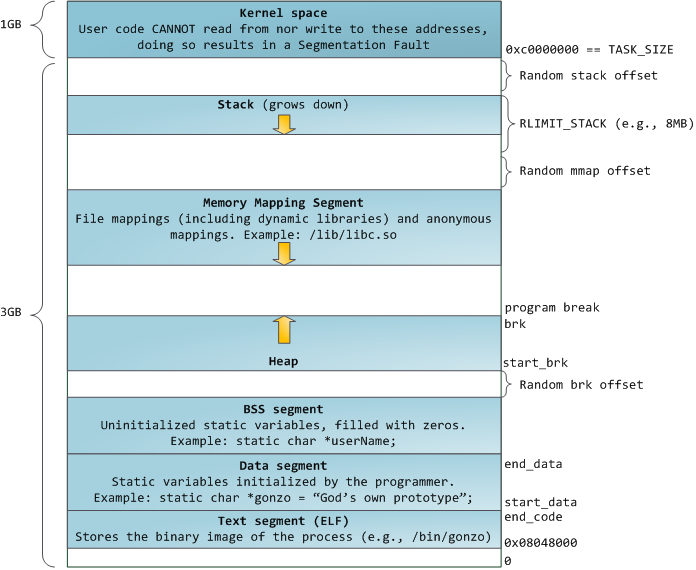
\includegraphics[width=10cm]{process_layout}
	\caption{Processo in memoria}
\end{figure}

La libreria standard del linguaggio C consente di interagire con l'heap mediante due funzioni:
\begin{lstlisting}[style=CStyle]
void* malloc(size_t size)
\end{lstlisting}
che alloca in heap uno spazio di dimensione \verb+size+ byte, e
\begin{lstlisting}[style=CStyle]
void free(void* p)
\end{lstlisting}
che dealloca dall'heap la zona di memoria puntata da \verb+p+, precedentemente allocata da \verb+malloc+.

Come si vedrà in seguito, se non vengono rispettate alcune regole, è possibile sfruttare le vulnerabilità per far eseguire ad un programma delle istruzioni arbitrarie da parte di un attaccante.